


%\renewcommand{\thechapter}{A}  % use A, B, C for chapter numbers
%\renewcommand{\chaptername}{Paper} % A chapter is now called Paper
%\renewcommand\thesection{\arabic{section}}
%\renewcommand*{\thepage}{A\arabic{page}}
%\setcounter{page}{1}
%\setcounter{section}{0}

%%% Paper content

\chapter{
	\centering{A Hierarchical Grocery Store Image Dataset with Visual and Semantic Labels}
}
\chaptermark{Hierarchical Grocery Store Image Dataset}
\vspace{-1cm}
\large{\textbf{Marcus Klasson}} \\
\large{\textit{Robotics, Perception, and Learning, EECS}} \\
\large{\textit{KTH Royal Institute of Technology, Stockholm, Sweden}} \\

\noindent\large{\textbf{Cheng Zhang}} \\
\large{\textit{Microsoft Research}} \\
\large{\textit{Cambridge, United Kingdom}} \\

\noindent\large{\textbf{Hedvig Kjellstr\"{o}m}} \\
\large{\textit{Robotics, Perception, and Learning, EECS}} \\
\large{\textit{KTH Royal Institute of Technology, Stockholm, Sweden}} 
%\begin{center}
%	\large{Marcus Klasson, Cheng Zhang, Hedvig Kjellström} \\
%	\small{HGej hej}
%\end{center}
\vspace{5pt}


%%%%%%%%%%%%%%%%%%%%%%%%%%%%%%%%%%%%%%%%%%%%%%%%%%%%%%%%%%%%%%%%%%%%%%%%%%%%%%%%
%%%%%%%%%%%%%%%%%%%%%%%%%%%%%%%%%%%%%%%%%%%%%%%%%%%%%%%%%%%%%%%%%%%%%%%%%%%%%%%%
\begin{abstract}
	Image classification models built into visual support systems and other assistive devices need to provide accurate predictions about their environment. We focus on an application of assistive technology for people with visual impairments, for daily activities such as shopping or cooking. In this paper, we provide a new benchmark dataset for a challenging task in this application -- classification of fruits, vegetables, and refrigerated products, e.g. milk packages and juice cartons, in grocery stores. To enable the learning process to utilize multiple sources of structured information, this dataset not only contains a large volume of natural images but also includes the corresponding information of the product from an online shopping website. Such information encompasses the hierarchical structure of the object classes, as well as an iconic image of each type of object. This dataset can be used to train and evaluate image classification models for helping visually impaired people in natural environments. Additionally, we provide benchmark results evaluated on pretrained convolutional neural networks often used for image understanding purposes, and also a multi-view variational autoencoder, which is capable of utilizing the rich product information in the dataset.
\end{abstract}

%%% Contents
\section{Introduction}\label{paperA:sec:introduction}

In this paper, we focus on the application of image recognition models implemented into assistive technologies for people with visual impairments. Such technologies already exist in the form of mobile applications, e.g.~Microsoft's Seeing AI \citeA{seeingAImicrosoft} and Aipoly Vision \citeA{aipolyvision}, and as wearable artificial vision devices, e.g.~Orcam MyEye \citeA{orcam} and the Sound of Vision system introduced in \citeA{paperA:caraiman2017soundofvision}. These products have the ability to support people with visual impairments in many different situations, such as reading text documents, describing the user's environment and recognizing people the user may know. 

\begin{figure}[t]
	\centering
    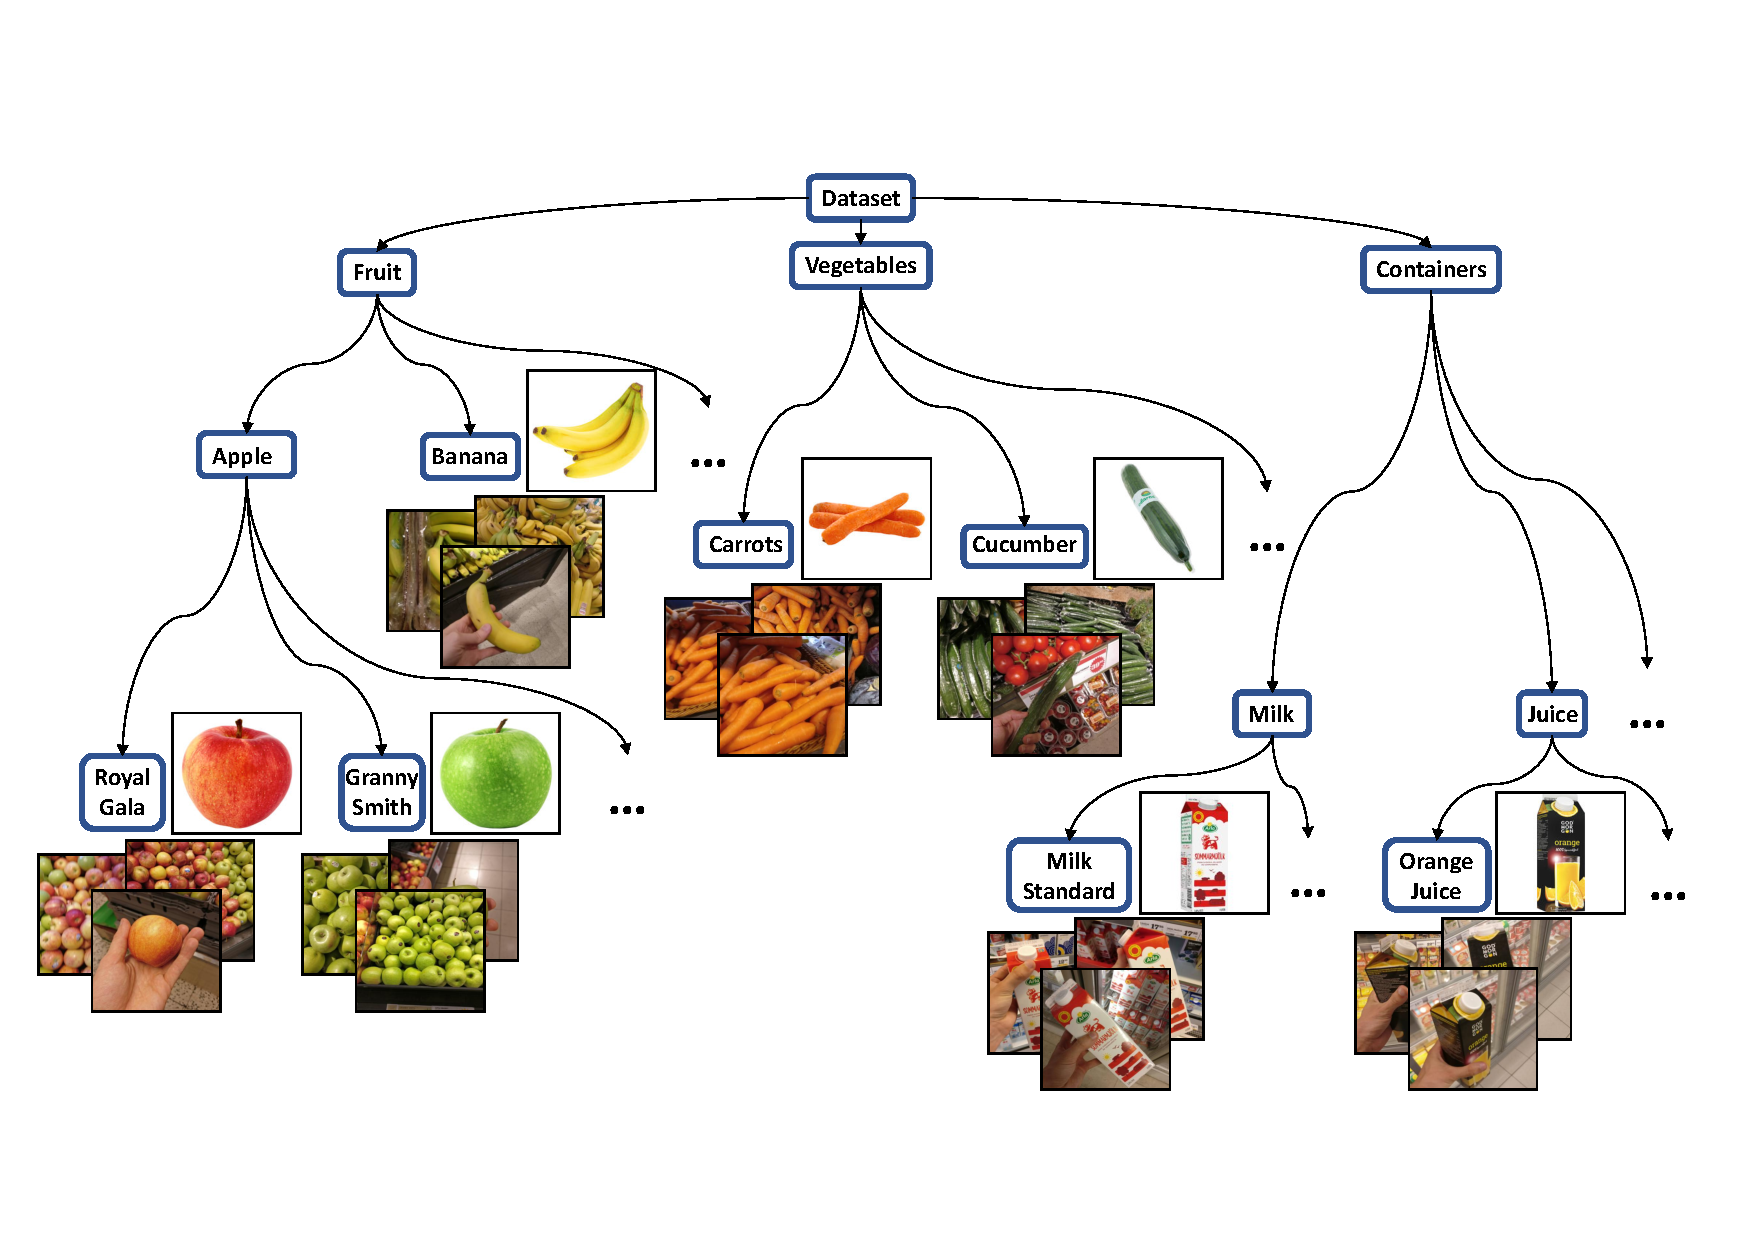
\includegraphics[width=0.9\textwidth]{PaperA/figures/intro.pdf}
    \vspace{-2mm}
    \caption{The primary contribution of this paper is a dataset of grocery items, for the purpose of training a visual recognition system to aid visually impaired people. The dataset is organized according to a hierarchical class structure, as illustrated above. A novel aspect of the dataset is that each class, apart from the semantic label, also has a visual label in the form of an iconic image.}
    \label{fig:examples} 
    \vspace{-3mm}
\end{figure}

We here address a complementary scenario not handled by current systems on the market: visual support when shopping for grocery items considering a large range of eatable objects, including fruits, vegetables, milk, and juices. 
In the case of fruits and vegetables, these are usually stacked in large bins in grocery stores as shown in Figure \ref{fig:dataset-figure}(a-f). A common problem in grocery stores is that similar items are often stacked next to each other; therefore, items are often misplaced into neighboring bins. Figure \ref{subfig:real-image-a} shows a mix of red and green apples, where it might be difficult for the system to determine which kind of apple is the actual target.
Humans can distinguish between groceries without vision to some degree, e.g.~by touching and smelling them, but it requires prior knowledge about texture and fragrance of food items.

Moreover, in addition to raw grocery items, there are also items that can only be differentiated with the help of visual information, e.g. milk, juice, and yogurt cartons, see Figure \ref{fig:dataset-figure}(g-i). Such items usually have barcodes, that are readable using the existing assistive devices described above. However, the barcodes are not easily located by visually impaired persons. Thus, an assistive vision device that fully relies on natural image understanding would be of significant added value for a visually impaired person shopping in a grocery store.

Image recognition models used for this task typically require training images collected in similar environments. However, current benchmark datasets, such as ImageNet \citeA{paperA:deng2009imagenet} and CIFAR-100 \citeA{paperA:Krizhevsky2009cifar100}, do contain images of fruits and vegetables, but are not suitable for this type of assistive application, 
since the target objects are commonly not presented in this type of natural environments, with occlusion and cluttered backgrounds. To address this issue, we present a novel dataset containing natural images of various raw grocery items and refrigerated products, e.g. milk, juice, and yogurt, taken in grocery stores. As part of our dataset, we collect images taken with single and multiple target objects, from various perspectives, and with noisy backgrounds.

In computer vision, previous studies have shown that model performance can be improved by extending the model to utilize other data sources, e.g. text, audio, in various machine learning tasks \citeA{paperA:frome2013DeVISE, paperA:Gebru2017FineGrainedCD, paperA:karpathy2015deepvisualsemantic, paperA:ngiam2011multimodal}. Descriptions of images are rather common to computer vision datasets, e.g. Flickr30k \citeA{paperA:plummer2015flickr30k}, whereas the datasets in \citeA{paperA:Gebru2017FineGrainedCD, paperA:Lin2014MicrosoftCoco} includes both descriptions and a reference image with clean background to some objects. Therefore, in addition to the natural images, we have collected iconic images with a single object centered in the image (see Figure \ref{fig:clean-image-figure}) and a corresponding product description to each grocery item. In this work, we also demonstrate how we can benefit from using additional information about the natural images by applying the multi-view generative model.

To summarize, the contribution of this paper is a dataset of natural images of raw and refrigerated grocery items, which could be used for evaluating and training image recognition systems to assist visually impaired people in a grocery store. 
The dataset labels have a hierarchical structure with both coarse- and fine-grained classes (see Figure \ref{fig:examples}). Moreover, 
each class also has an iconic image and a product description, which makes the dataset applicable to multimodal learning models. The dataset is described in Section \ref{paperA:sec:our_dataset}. 

We provide multiple benchmark results using various deep neural networks, such as Alexnet \citeA{paperA:krizhevsky2012imagenet}, VGG \citeA{paperA:simonyan2014verydeep}, DenseNet \citeA{paperA:huang2017densely}, as well as deep generative models, such as VAE \citeA{paperA:kingma2014autoencoding}. 
Furthermore, we adapt a multi-view VAE model to make use of the iconic images for each class (Section \ref{paperA:sec:classification_methods}), and show that it improves the classification accuracy given the same model setting (Section \ref{paperA:sec:experimental_results}). Last, we discuss possible future directions for fully using the additional information provided with the dataset and adopt more advanced machine learning methods, such as visual-semantic embeddings, to learn efficient representations of the images. 
\begin{comment}


\begin{figure*}[t] 
\centering
\begin{minipage}[t]{0.47\textwidth}
\centering
\subfigure[Royal Gala]{\label{subfig:real-image-a}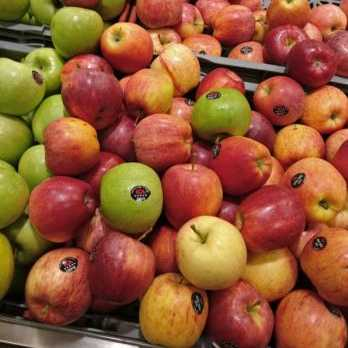
\includegraphics[width=0.30\columnwidth]{PaperA/dataset-figure/Royal-Gala-Apple_84_crop.jpg}}~
\subfigure[Golden Delicious]{\label{subfig:real-image-c}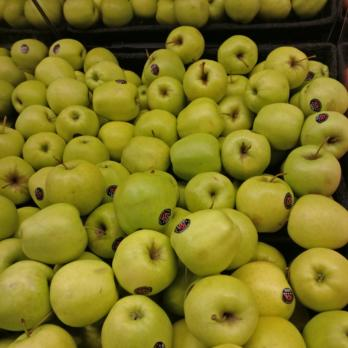
\includegraphics[width=0.30\columnwidth]{PaperA/dataset-figure/Golden-Delicious-Apple_7.jpg}}~
\subfigure[Orange]{\label{subfig:real-image-f}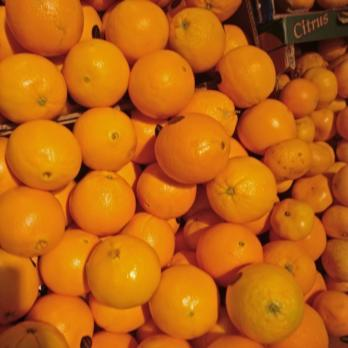
\includegraphics[width=0.30\columnwidth]{PaperA/dataset-figure/Orange_025.jpg}}~ \\ %\vspace{0.2cm}
\subfigure[Aubergine]{\label{subfig:real-image-h}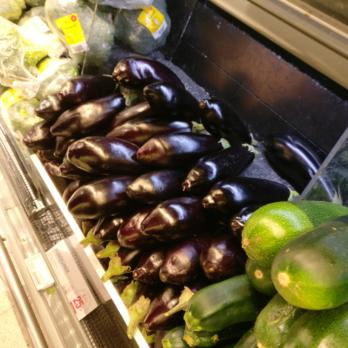
\includegraphics[width=0.30\columnwidth]{PaperA/dataset-figure/Aubergine_016.jpg}}~
\subfigure[Onion]{\label{subfig:real-image-j}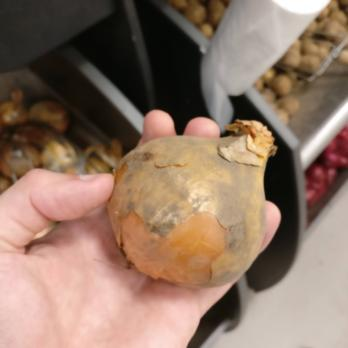
\includegraphics[width=0.30\columnwidth]{PaperA/dataset-figure/Yellow-Onion_25.jpg}}~
\subfigure[Zucchini]{\label{subfig:real-image-l}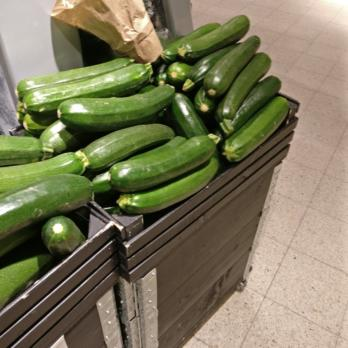
\includegraphics[width=0.30\columnwidth]{PaperA/dataset-figure/Zucchini_015.jpg}}~ \\ %\vspace{0.2cm}
\subfigure[Apple Juice]{\label{subfig:real-image-n}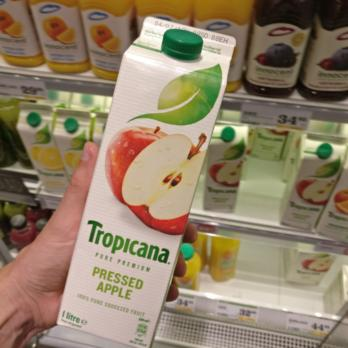
\includegraphics[width=0.30\columnwidth]{PaperA/dataset-figure/Tropicana-Apple-Juice_16.jpg}}~
\subfigure[Milk Medium Fat]{\label{subfig:real-image-q}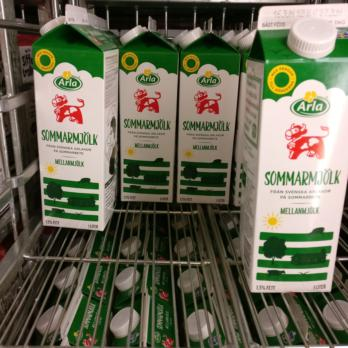
\includegraphics[width=0.30\columnwidth]{PaperA/dataset-figure/Arla-Milk-Medium-Fat_17.jpg}}~
\subfigure[Yogurt Natural]{\label{subfig:real-image-r}
\includegraphics[width=0.30\columnwidth]{PaperA/dataset-figure/Arla-Natural-Yoghurt_031.jpg}}~
   \caption{Examples of natural images in our dataset, where each image have been taken inside a grocery store. Image examples of fruits, vegetables and refrigerated products are presented in each row respectively.
   }
\label{fig:PaperA/dataset-figure}
\end{minipage}
\hspace{10pt}
\begin{minipage}[t]{0.47\textwidth}
\vspace{0pt}
\centering
\subfigure[Royal Gala]{\label{subfig:clean-img-a}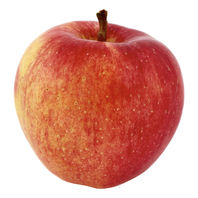
\includegraphics[width=0.30\columnwidth]{PaperA/clean-image-figure/Royal-Gala-Apple_Clean.jpg}}~
\subfigure[Golden Delicious]{\label{subfig:clean-img-c}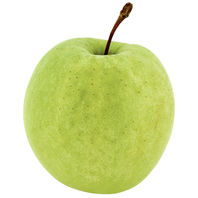
\includegraphics[width=0.30\columnwidth]{PaperA/clean-image-figure/Golden-Delicious-Apple_Clean.jpg}}~
\subfigure[Orange]{\label{subfig:clean-img-f}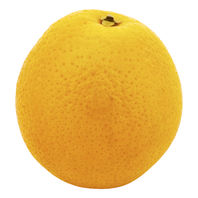
\includegraphics[width=0.30\columnwidth]{PaperA/clean-image-figure/Orange_Clean.jpg}}~ \\ %\vspace{-0.2cm}
\subfigure[Aubergine]{\label{subfig:clean-img-h}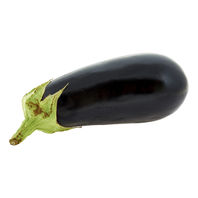
\includegraphics[width=0.30\columnwidth]{PaperA/clean-image-figure/Aubergine_Clean.jpg}}~
\subfigure[Onion]{\label{subfig:clean-img-j}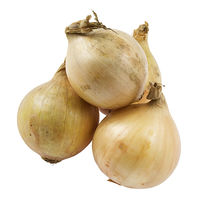
\includegraphics[width=0.30\columnwidth]{PaperA/clean-image-figure/Yellow-Onion_Clean.jpg}}~
\subfigure[Zucchini]{\label{subfig:clean-img-l}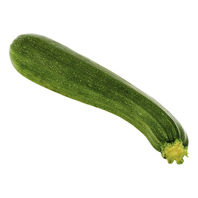
\includegraphics[width=0.30\columnwidth]{PaperA/clean-image-figure/Zucchini_Clean.jpg}}~ \\ %\vspace{-0.2cm}
\subfigure[Apple Juice]{\label{subfig:clean-img-n}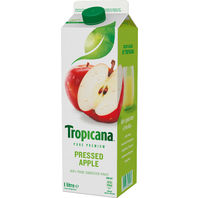
\includegraphics[width=0.30\columnwidth]{PaperA/clean-image-figure/Tropicana-Apple-Juice_Clean.jpg}}~
\subfigure[Milk Medium Fat]{\label{subfig:clean-img-q}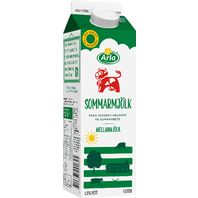
\includegraphics[width=0.30\columnwidth]{PaperA/clean-image-figure/Arla-Milk-Medium-Fat_Clean.jpg}}~
\subfigure[Yogurt Natural]{\label{subfig:clean-img-r}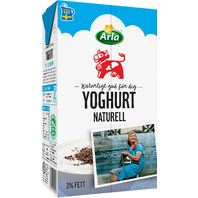
\includegraphics[width=0.30\columnwidth]{PaperA/clean-image-figure/Arla-Natural-Yoghurt_Clean.jpg}}~
   \caption{Examples of iconic images downloaded from a grocery shopping website, which corresponds to the target items in the images in Figure \ref{fig:PaperA/dataset-figure}.}
\label{fig:PaperA/clean-image-figure}
\end{minipage}
\end{figure*}
\end{comment}

\section{Related Work}\label{sec:related-work}

Many popular image datasets have been collected by downloading images from the web \citeA{deng2009imagenetPaperA,Everingham2010pascal,Gebru2017FineGrainedCD, griffin2007caltech256,Krizhevsky2009cifar100,Lin2014MicrosoftCoco, song2016deep, welinder2010birds,xiao2010sundatabase}. 
If the dataset contains a large amount of images, it is convenient to make use of crowdsourcing to get annotations for recognition tasks \citeA{deng2009imagenetPaperA,Krizhevsky2009cifar100,liu2015faceattributes}. For some datasets, the crowdsourcers are also asked to put bounding boxes around the object to be labeled for object detection tasks \citeA{Everingham2010pascal,Gebru2017FineGrainedCD,welinder2010birds}. In \citeA{griffin2007caltech256} and \citeA{Krizhevsky2009cifar100}, the target objects are usually centered and takes up most content of the image itself. Another significant characteristic is that web images usually are biased in the sense that they have been taken with the object focus in mind; they have good lighting settings and are typically clean from occlusions, since the collectors have used general search words for the object classes, e.g. \textit{car}, \textit{horse}, or \textit{apple}.

Some datasets include additional information about the images beyond the single class label, e.g. text descriptions of what is present in the image and bounding boxes around objects. These datasets can be used in several different computer vision tasks, such as image classification, object detection, and image segmentation. Structured labeling is another important property of a dataset, which provides flexibility when classifying images. In  \citeA{Gebru2017FineGrainedCD,Lin2014MicrosoftCoco}, all of these features exist and moreover they include reference images to each object class, which in \citeA{Lin2014MicrosoftCoco} is used for labeling multiple  categories present in images, while in \citeA{Gebru2017FineGrainedCD} these images are used for fine-grained recognition. 
Our dataset includes a reference image, i.e. the iconic image, and a product description for every class, and we have also labeled the grocery items in a structured manner.

Other image datasets of fruits and vegetables for classification purposes are the FIDS30 database \citeA{marko2013fids30} and the dataset in \citeA{muresan2017fruit}. The images in FIDS30 were downloaded from the web and contain background noise as well as single or multiple instances of the object. In \citeA{muresan2017fruit}, all pixels belonging to the object are extracted from the original image, such that all images have white backgrounds with the same brightness condition. There also exist datasets for detecting fruits in orchards for robotic harvesting purposes, which are very challenging since the images contain plenty of background and various lighting conditions, and the targeted fruits are often occluded or of the same color as the background \citeA{bargoti2017deepfruitdetection,sa2016deepfruits}.

Another dataset that is highly relevant to our application need is presented in  \citeA{waltner2015mango}. They collected a dataset for training and evaluating the image classifier by extracting images from video recordings of 23 main classes, which are subdivided into 98 classes, of raw grocery items (fruits and vegetables) in different grocery stores. Using this dataset, a mobile application was developed to recognize food products in grocery store environments, which provides the user with details and health recommendations about the item along with other proposals of similar food items. For each class, there exists a product description with nutrition values to assist the user in shopping scenarios. The main difference between this work and our dataset is firstly the clean iconic images (visual labels) for each class in our dataset, and secondly that we have also collected images of refrigerated items, such as dairy and juice containers, where visual information is required to distinguish between the products.   


\renewcommand*{\bibname}{References}
\bibliographystyleA{unsrt}
\bibliographyA{References/paperA}
